\chapter{Preliminaries}
\label{chap:matint}
\vspace*{-0.9cm}

% \startcontents[chapters]
% \printcontents[chapters]{}{1}{}

The goal of this text is nothing more but a short \textbf{very informal} introduction to algebraic topology, focussed on introducing useful techniques from maths for determining algebraic invariants which are of physical significance.

\section{Homeomorphisms}
In the past, I noticed that words as \emph{homeomorphism}, \emph{diffeomorphism}, \emph{homotopy equivalence} and \emph{homotopy} get mixed up, so I want to make their differences clear and motivate them. I think this becomes especially clear if one considers categories and functors between them to understand those definitions, but we can be more explicit. We start with a topological setup:
\begin{definition}[Topological Space]
\marginnote{
    One should think of topological spaces as generalizations of metric spaces. In metric spaces like $\mathbb{R}^n$, open subsets are determined by the Euclidean metric. If one thinks about the properties such open subsets satisfy, (T1)-(T3) are almost immediate. For example, take $\mathbb{R}$ with the usual topology $$\mathcal{T}:=\{U \subseteq \mathbb{R} \mid \forall x \in U \exists \epsilon > 0: (x-\epsilon, x+\epsilon) \in U\}.$$ For all $x \in \mathbb{R}$, we can take $\epsilon =1$ and have $(x-1,x+1) \subseteq \mathbb{R}$, so $\mathbb{R} \in \mathcal{T}$. For the empty set, the statement is vacuously true, so $\emptyset \in \mathcal{T}$. If $\{U_i\}_{i\in I}$ is a (possibly uncountably infinite) family of open subsets of $\mathbb{R}$ and $x \in \cup_{i \in I} U_i$, by definition we have $x \in U_\alpha$ for some $\alpha \in I$. This means that there is $\epsilon >0$ such that $(x- \epsilon, x+\epsilon) \subseteq U_\alpha$ since all $U_i$ are open. But then we have $(x-\epsilon, x+\epsilon) \subseteq \cup_{i \in I} U_i$ by definition of the union. Lastly, given $U_1,U_2 \in \mathcal{T}$ and $x \in U_1 \cap U_2$, we can find $\epsilon_1, \epsilon_2 > 0$ such that $(x-\epsilon_i, x+\epsilon_i) \subseteq U_i$. But then we have $(x-\epsilon, x+\epsilon) \subseteq U_1 \cap U_2$ for $\epsilon = \min\{\epsilon_1,\epsilon_2\}$. 
}
    A \textbf{topology} on a set $X$ is a family $\mathcal{T}$ of subsets of $X$ such that:
    \begin{enumerate}[({T}1)]
        \item $X \in \mathcal{T}$ and $\emptyset \in \mathcal{T}$
        \item If $I$ is an arbitrary indexing family and $\forall i \in I: U_i \in \mathcal{T}$, we also have $$\bigcup_{i \in I} U_i \in \mathcal{T}$$
        \item For all $U,V \in \mathcal{T}$, $U \cap V \in \mathcal{T}$.
    \end{enumerate}
    Then, we call $\mathcal{T}$ \textbf{topology} on $X$ and $(X,\mathcal{T})$ \textbf{topological space}. The sets $U \in \mathcal{T}$ are called \textbf{open sets} of $X$.
\end{definition}
\begin{eg}
    There are many important examples:
    \begin{itemize}
        \item Every metric space is a topological space by taking the topology to be induced by the metric. This makes $\mathbb{R}^n$ and $\mathbb{C}^n$ topological spaces in particular. Since subsets of metric spaces are metric, those are also topological spaces.
        \item \marginnote{Note two things here: Firstly, being a topological space is really not difficult. However, having an actually useful topology is a whole different story. Secondly, topologies are clearly not unique: We can give $\mathbb{R}^n$ the metric topology, but also the discrete or the indiscrete topology. The obvious choice is of course the first one, which is why we call it canonical.} Every set can be turned into a topological space by declaring all possible subsets of that set to be open. This is called the \textbf{discrete topology}.
        \item Similarly, we can take any set $X$ and define a topology by saying $X$ and $\emptyset$ are the only open sets. This is the \textbf{indiscrete topology}.  
    \end{itemize}
\end{eg}
In physics, one often only deals with topologies induced by a metric, so feel free to take $\mathbb{R}^n$ as playground for imagination. Now we have sets with new structure, but there is no reason why a function $f: X \to Y$ should preserve this stucture, i.e. there is no reason for $f^{-1}(V)$ to be open in $X$ even if $V$ is open in $Y$.
\begin{definition}[Continuity]
    A function $f: X \to Y$ between topological spaces is continuous if for all open subsets $V$ of $Y$, $f^{-1}(V)$ is open in $X$. 
\end{definition}
For the usual metric spaces, this agrees with the $\epsilon$-$\delta$-definition of continuity.
For two sets $A,B$, we said that $A \cong B$, or $A$ isomorphic to $B$, if there is a bijective map between $A$ and $B$. We want to extend this to topological spaces with their additional structure:
\begin{definition}[Homeomorphism]
    A function $f: (X, \mathcal{T}) \to (Y, \mathcal{T}')$ is called \textbf{homeomorphism} if $f$ is bijective and $f$ as well as $f^{-1}$ are continuous. In this case, we write $(X, \mathcal{T}) \cong (Y, \mathcal{T}')$ and say that $X$ and $Y$ are \textbf{homeomorphic} or \textbf{isomorphic as top. spaces}.
\end{definition}
This means when we think about topological spaces, continuous functions with continuous inverses are all we could ask for: They preserve all topological structure. Intuitively, one has to take care of two things: The map cannot tear or crease as it is continuous, and it has to be bijective, so no information should be lost.
\begin{eg}
\begin{marginfigure}
    \centering
    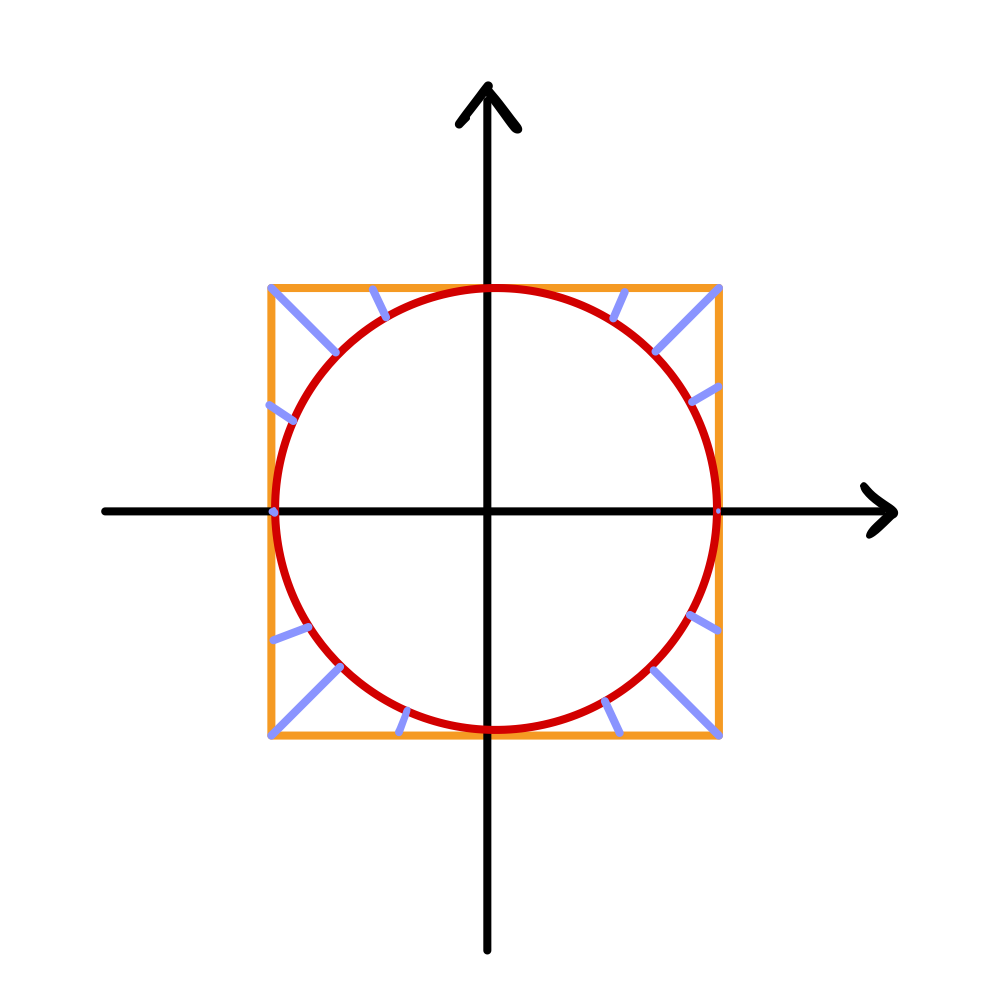
\includegraphics[scale=.15]{figures/blowup.png}
    \caption{A circle can be blown up to a square and a square can be shrunken down to a circle. This is a homeomorphism.}
\end{marginfigure}
    \begin{itemize}
        \item Every open interval $(a,b) \subseteq \mathbb{R}$ is homeomorphic to $\mathbb{R}$ itself. We can always blow it up or shrink it down as necessary.
        \item Charts of manifolds are homeomorphisms, so every manifold is \textbf{locally} homeomorphic to $\mathbb{R}^n$.
        \item A point $x \in \mathbb{R}$ can never be homeomorphic to some open interval in $\mathbb{R}$ since there cannot exist a bijection between a finite and an uncountably infinite set. Similarly, $\mathbb{S}^1$ cannot be homeomorphic to an open interval as $\mathbb{S}^1$ is compact while open intervals are not.
        \item Size is not a topological property: All open balls of $\mathbb{R}^n$ are homeomorphic by translation $x \mapsto x+y$ or dilation $x \mapsto \lambda x$.
    \end{itemize}
\end{eg}
We conclude this digression with probably the most intricate definition:
\begin{definition}[Topological Embedding]
    \marginnote{
        One should think of an embedding as having a true copy of $S$ inside of $X$ such that the topology of $S$ as a subset of $X$ (which is obviously induced by the topology on $X$) agrees with the original topology of $S$ as a topological space.
    }
    Let $S,X$ be topological spaces and $f: S \to X$ be a function. We call $f$ \textbf{topological embedding} if $f$ is injective and the restriction $$\tilde{f}:S \to f(S) \subseteq X$$ is a homeomorphism.
\end{definition}
\begin{eg}
    \begin{itemize}
        \item The graph of the parabola given by $$F: \mathbb{R} \to \mathbb{R}^2, \, x \mapsto (x, x^2)$$ is an embedding: It is injective everywhere and on the image of $F$, we can use the projection $(x,y) \mapsto x$ as inverse map. Both $F$ and the projection are clearly continuous.
        \item Every topological manifold of dimension $n$ can be embedded into some $\mathbb{R}^N$ for $N$ large enough. Hence every manifold is a submanifold (\emph{Whitney embedding theorem}).
        \item The lemniscate (figure 8), given as $$G: [0,1] \to \mathbb{C}, \, t \mapsto \exp(2 \pi i t),$$ is not an embedding as it fails to be injective: $G(0)=G(1)$. Removing the problematic self-intersection, $$G': [0,1) \to \mathbb{C}$$ is still not an embedding as the metric topology on $\mathbb{C}$ does not agree with the topology of $G'([0,1))$. This is a good example for why embeddings are sometimes a bit tricky. The good news is that restriction on any smaller interval $[0,a)$ with $a < 1$ will also solve this problem, turning the open lemniscate into a topological subspace of $\mathbb{C}$.
    \end{itemize}
\end{eg}
We can now collect the first result about the problem at hand.
\begin{prop}
   The map 
   \begin{align}
       F:  \mathbb{S}^1 \times \mathbb{S}^1 &\to \mathbb{R}^3\\
       (u,v,w,z) &\mapsto (u+w, v, z)
   \end{align}
   fails to be an embedding.
\end{prop}
\begin{proof}
    Consider the complex numbers $(1,0)$ and $(-1,0)$ which are clearly on the unit circle $\mathbb{S}^1 \subseteq \mathbb{C}$. Then, we have: 
    \begin{equation*}
        F((1,0),(-1,0))=(0,0,0)=F((-1,0),(1,0)),
    \end{equation*}
    and hence $F$ is not injective.
\end{proof}
\section{Algebraic Invariants and the Fundamental Group}
Homeomorphisms are great. They preserve all possible topological structure. However, they are also often very difficult or do not exist at all between two given spaces. Therefore, we want to look for means to compare topological spaces that are less strict, but still fine enough to be actually useful. In practice, we are looking for algebraic invariants: Informally speaking, algebraic invariants are algebraic objects we can assign to a topological space which are preserved under some kind of map. This makes it possible to characterize spaces in regard to some designated property, stripping the space of all unnecessary data for the problem at hand. Those invariants often come in the form of special numbers (e.g. Euler characteristic) or groups.


\begin{marginfigure}
    \centering
    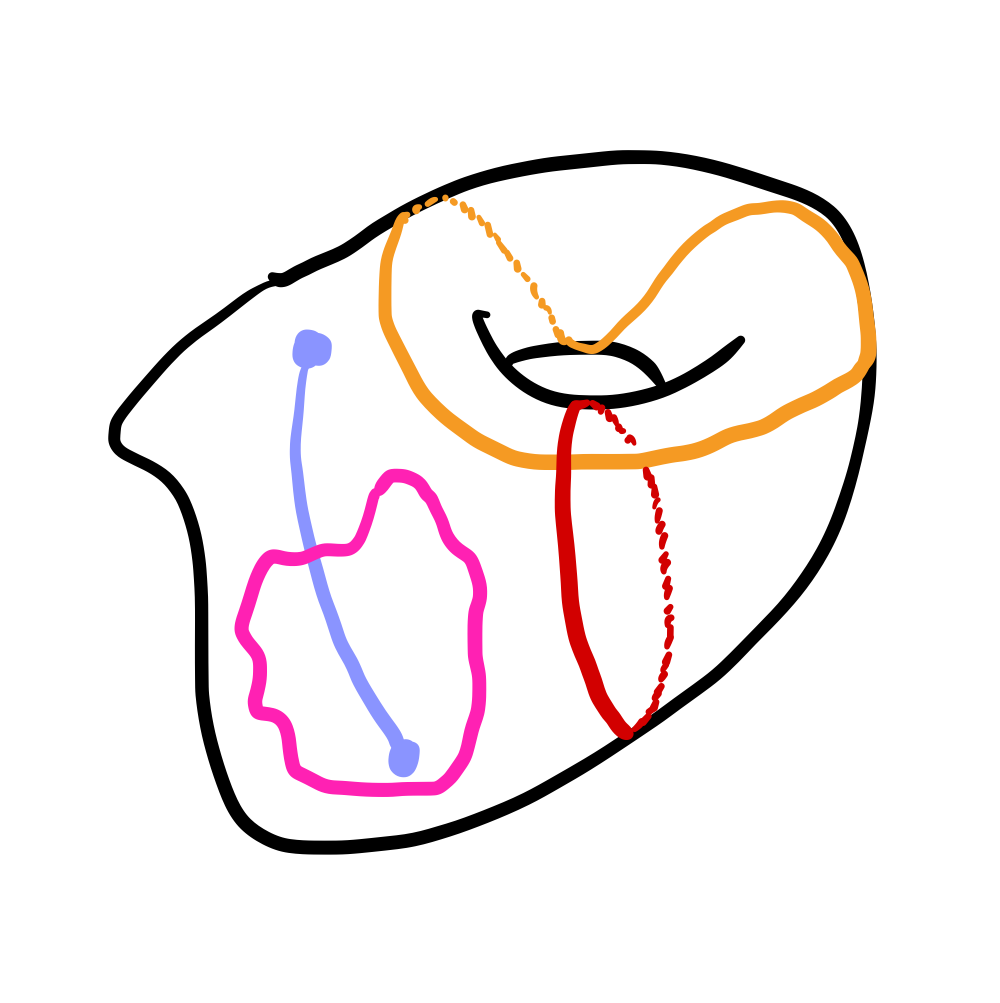
\includegraphics[scale=.08]{figures/paths.png}
    \caption{Some open and closed paths in a space homeomorphic to a torus.}
\end{marginfigure}
\begin{definition}[Path]
    Let $X$ be a topological space. A \textbf{path} in $X$ is a continuous map $$\gamma: [0,1] \to X.$$ We say that $\gamma$ is closed if $\gamma(0)=\gamma(1)$, or equivalently, $\gamma$ is a continuous map $\mathbb{S}^1 \to X$.
\end{definition}
Our goal is to detect fundamental properties of spaces with paths. One can immediately think of holes: Somehow, the main difference between the torus and a sphere should be that the torus has a hole, while the sphere does not. Which kind of map does preserve at least holes?

\begin{marginfigure}
    \centering
    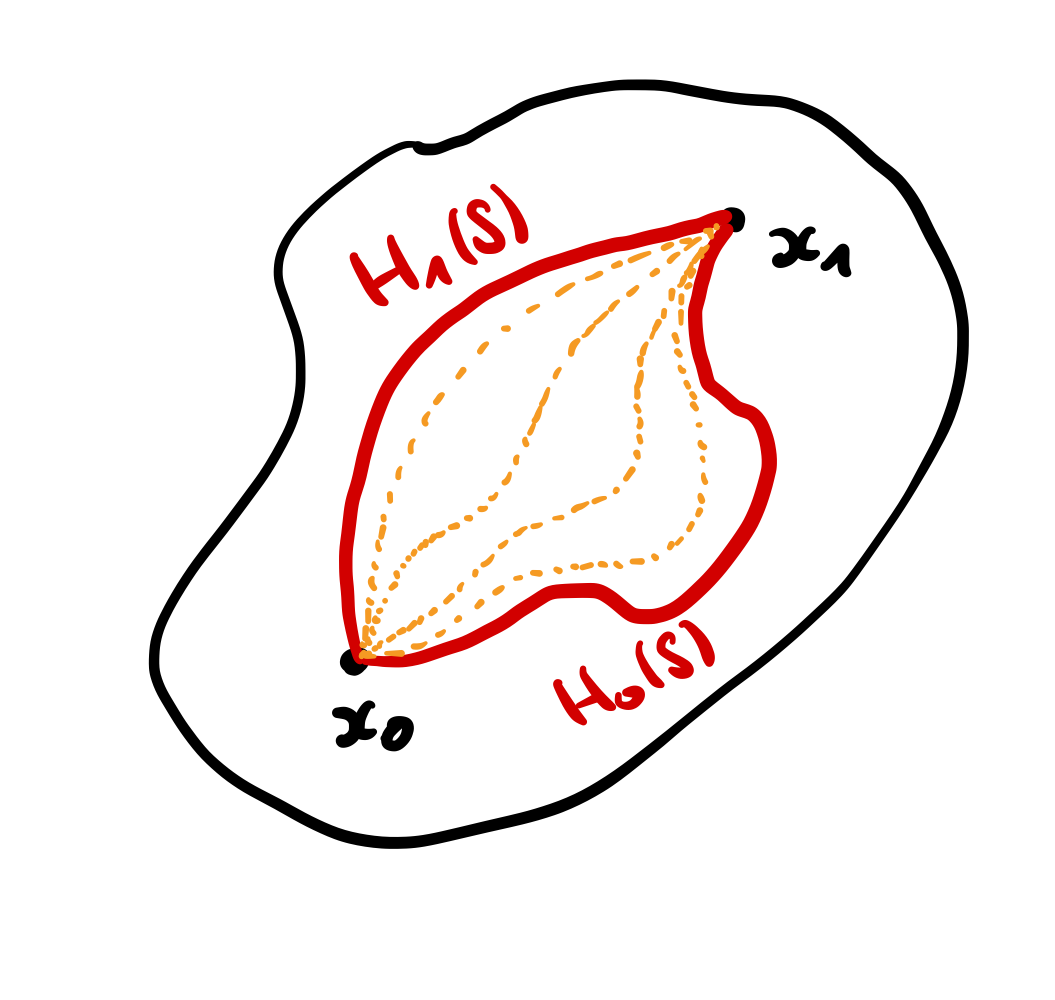
\includegraphics[scale=.1]{figures/homotopy.png}
    \caption{A continuous path homotopy with fixed endpoints.}
\end{marginfigure}
\begin{definition}[Path homotopy]
    Two paths $\gamma, \omega: [0,1] \to X$ are \textbf{path-homotopic} if $\gamma(0)=\omega(0)=:x_0$, $\gamma(1)=\omega(1)=:x_1$, and there is a continuous map $$H: [0,1] \times [0,1] \to X$$ with:
    \begin{itemize}
        \item $H(s,0)=H_0(s)=\gamma(s)$
        \item $H(s,1)=H_1(s)=\omega(s)$
        \item $H(0,t)=H_t(0)=x_0$
        \item $H(1,t)=H_t(1)=x_1$
    \end{itemize}
    We call $H$ a \textbf{path homotopy} and write $\gamma \simeq \omega$.
\end{definition}
\begin{eg}
    Consider the punctured plane $\mathbb{R}^2 \setminus \{0\}$. The paths $\gamma_1(t):=(\cos \pi t, \sin \pi t)$ and $\gamma(t):=(\cos \pi t, n \cdot \sin \pi t)$ are path-homotopic for all $n > 0$. One just connects $\gamma_1$ and $\gamma_2$ by straight lines and slides all points along them. This is a homotopy. However, $\gamma_1$ is never homotopic to $\gamma_3(t):=(\cos \pi t, - \sin \pi t)$, as every homotopy would have to pass through the origin, which was removed by assumption.
\end{eg}
This should give a hunch about why homotopies discern certain paths. We are ready to define the first algebraic invariant:
\begin{definition}[Fundamental Group]
    Let $X$ be a topological space. The \textbf{fundamental group} of $X$ with base point $x_0 \in X$, written $\pi_1(X,x_0)$, is given by homotopy classes of closed paths $\mathbb{S}^1 \to X$.
\end{definition}
So if two paths have a homotopy between them, the fundamental group does treat them as the same path. Why is this a group? The proof is a bit annoying, but we do some heuristics: Two paths can be concatenated to a new path if the endpoint of the first path is the starting point of the second path. The inverse of a path is given by going backwards, i.e. reparametrizing $t \mapsto -t$, and the identity is just standing around, i.e. the constant path $\gamma(t)=x_0$.
We still need to know when two spaces are "identical enough" to have the same fundamental group. Previously, we defined a homotopy for paths. Now we consider general homotopies between continuous maps, which are almost identical apart from the fact that we do not demand fixed endpoints.
\begin{definition}[Homotopy Equivalence]
    Two topological spaces $X$ and $Y$ are said to be \textbf{homotopy equivalent} if there are maps $f: X \to Y$ and $g: Y \to X$ such that $f \circ g  \simeq \id_Y$ and $g \circ f \simeq \id_X$, where $\simeq$ means that there exists a homotopy (not necessarily a path-homotopy) between the left and the right side. We write $X \simeq Y$.
\end{definition}
So this is our criterion for the fundamental group to be equal:
\begin{prop}
 Let $X,Y$ be topological spaces, $x_0 \in X$, $y_0 \in Y$. The fundamental groups are isomorphic $$\pi_1(X,x_0) \cong \pi_1(Y,y_0)$$ if one of the following conditions holds:
 \begin{itemize}
     \item $X$ and $Y$ are homeomorphic.
     \item $X$ and $Y$ are homotopy equivalent. 
 \end{itemize}
\end{prop}
\marginnote{
    Every homeomorphism gives rise to a homotopy equivalence as the first one is much stronger, like we discussed. But when are homotopy eqivalences not homeomorphisms? This occurs often because of failure of bijectivity. One of the funniest examples is that the letter X and the letter Y are homotopy equivalent, but not homeomorphic. The equivalence is given by shortening one of the spikes of $X$ to the center of the letter X. This maps the letter X to Y. We map Y to X by mapping the three spikes of Y to three out of four spikes of X. Performing these moves in succession is just the identity, we end up with either X or Y. But the maps are very clearly non-surjective and non-injective.}

\begin{remark}
    In general, it is very difficult to calculate the fundamental group of a space from first principles. One famous example is the very annoying proof that $\pi_1(\mathbb{S}^1) \cong \mathbb{Z}$. As physicists, it is somewhat nice that we can use our intuition to infer some fundamental groups without giving a full proof.
\end{remark}
\begin{eg} 
    Whenever it is not of concern, we will suppress the basepoint in the notation of $\pi_1$
    \begin{itemize}
    \item The real space $\mathbb{R}^n$ has trivial fundamental group for all $n$. We call such spaces \textbf{simply connected}. Note: \emph{Even though $\pi_1(\mathbb{R}^n) \cong \pi_1(\mathbb{R}^m)$ for $n \neq m$, there can never be a homeomorphism $\mathbb{R}^n \to \mathbb{R}^m$ for $n \neq m$. This is an example where the fundamental group is not enough to predict topological equivalence.}
    \item $\pi_1{S^1} \cong \mathbb{Z}$: This is seen intuitively by realizing that there are only two fundamentally different closed paths in $\mathbb{S}^1$: One can take the constant path, which is ismorphic to $0 \in \mathbb{Z}$. \marginnote{Think of $\mathbb{Z}$ as abelian group under addition: The neutral element is $0$.} For all other paths, the only sensible difference is how often and in which direction one traverses the circe. Direction is mapped to the sign of the integer, and the amount of closed loops to the modulus.
    \item $\pi_1(\mathbb{S}^n)\cong \{0\}$ for all $n>1$. This is something to remember well: All spheres in dimension $2$ and higher are simply connected. For $\mathbb{S}^2$, one can imagine a rubber band sliding of a basketball to see the homotopy connecting every path to the trivial one.
    \item $\pi_1(\mathbb{S}^1 \times \cdots \times \mathbb{S}^1) \cong \mathbb{Z} \times \cdots \times \mathbb{Z}$: Remember that $\mathbb{S}^1 \times \mathbb{S}^1$ is the torus, so there are two fundamental paths in the torus and hence the fundamental group consists of two copies of the integers, one for each path.
    \item One shall not imagine all fundamental groups to be nicely abelian. Take the connected sum of two circles, $\mathbb{S}^1 \vee \mathbb{S}^1$. The fundamental group is $\mathbb{Z} \star \mathbb{Z}$, where $\star$ denotes the free product of groups. We will introduce this later. For now, note that the free product is very far from being abelian, i.e. commutative.
    \end{itemize}
\end{eg}
We will need another definition already mentioned: The paths I called fundamental (e.g. traversing $\mathbb{S}^1$ once, or traversing meridian and longitude of the torus once) are called \textbf{generators} of the fundamental group, since all other paths can be obtained by walking that path multiple times and/or reversing direction.\marginnote{There is indeed a connection between the fact that $\mathbb{S}^1$ has two generators differing only in sign and also two orientations induced by tangent vector fields.} Thinking abstractly, the generators of $\pi_1(\mathbb{S}^1) \cong \mathbb{Z}$ are just $\pm 1 \in \mathbb{Z}$.
\section{Homology}
If $\pi_1$ is too complicated, we could try to simplify it as a group. $\pi_1$ is pretty clearly non-abelian, so $\gamma_1 \ast \gamma_2 \neq \gamma_2 \ast \gamma_1$ in general. What happens if we just force all non-commuting paths to commute?\marginnote{This is done in group theory by abelianizing: We take the quotient of the non-abelian group by the subgroup generated by all elements of the form $aba^{-1}b^{-1}$.} Unfortunately, this is a bit more involved than defining $\pi_1$, but in return we get directly all homology groups, not only the first one.
\begin{marginfigure}
    \centering
    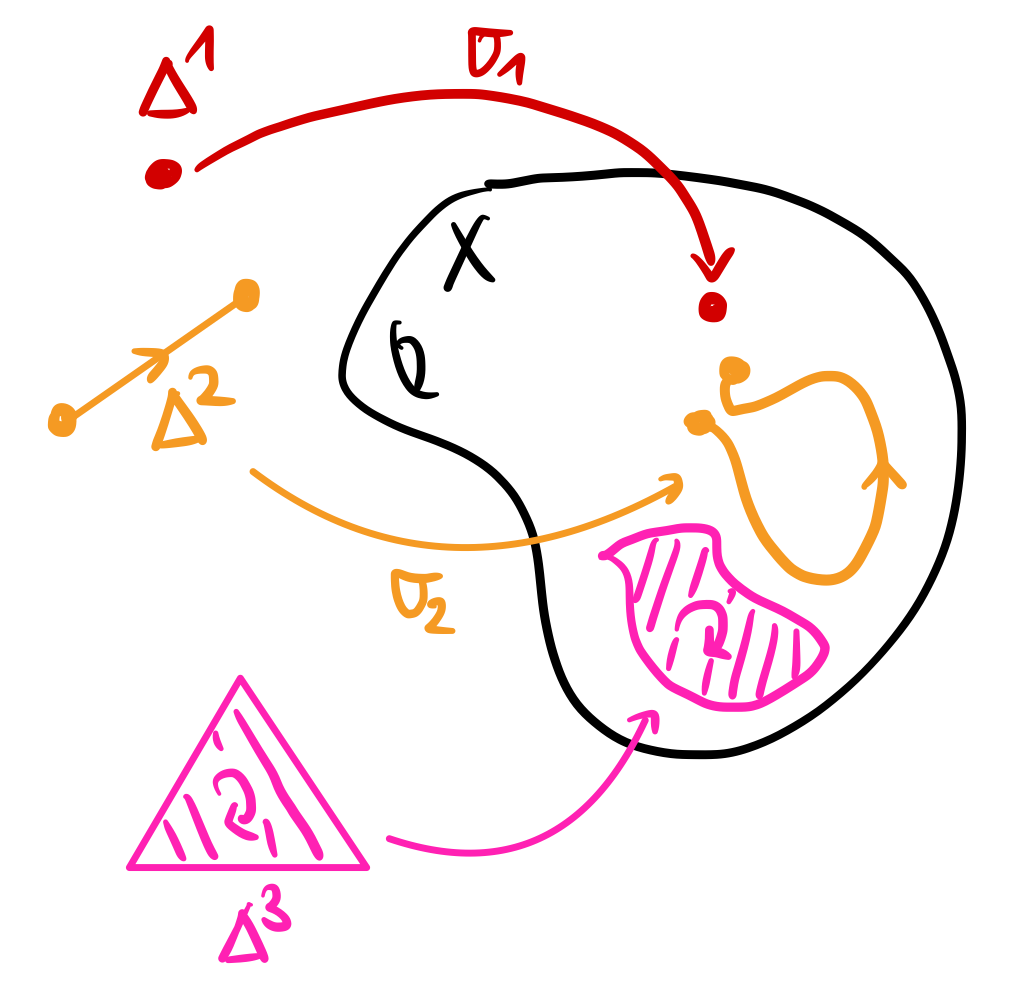
\includegraphics[scale=.08]{figures/simplex.png}
    \caption{Different singular simplices are mapped into a top. space $X$.}
\end{marginfigure}
We denote the $n$-simplex by $\Delta^n$. This is just a hypertriangle, if one wants to imagine it like that: For $n=1$, we have a point. For $n=2$, we have a straigt line, i.e. the interval $[0,1]$. For $n=3$, we have a filled-out triangle. For $n=4$, we have a filled-out tetrahedron, and so on. Given a top. space $X$, a \textbf{singular n-simplex} is a continuous map $$\sigma: \Delta^n \to X.$$ This means we just wiggle our $n$-simplex in our top. space without tearing or creasing. There is a map $\partial_n: \Delta^n \to \Delta^{n-1}$ for any $n$ which delets the interior of the $n$-simplex, leaving a sum of $n-1$-simplices. We call this the \textbf{face operator}.
\begin{figure}[H]
    \centering
    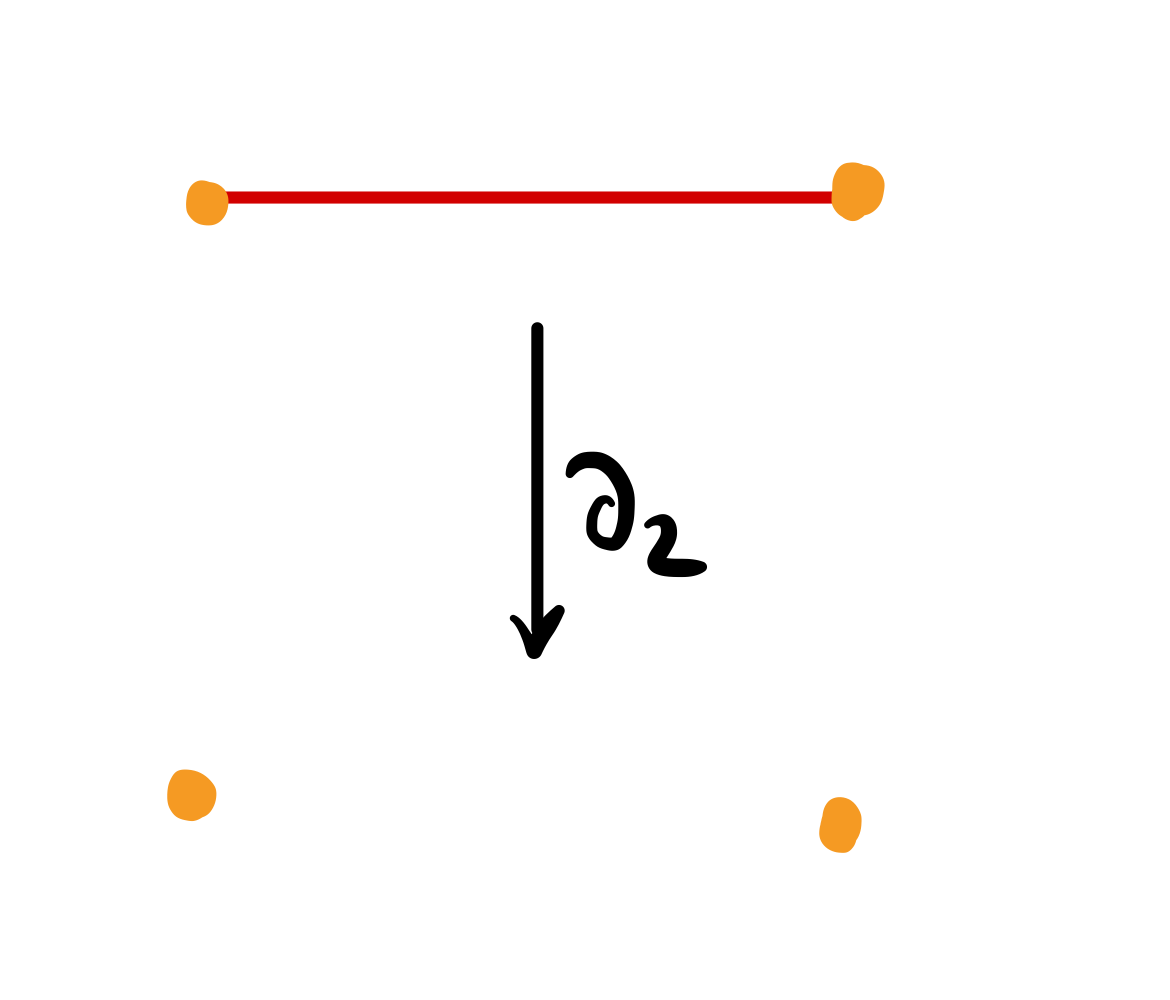
\includegraphics[scale=.08]{figures/twosimp.png}
    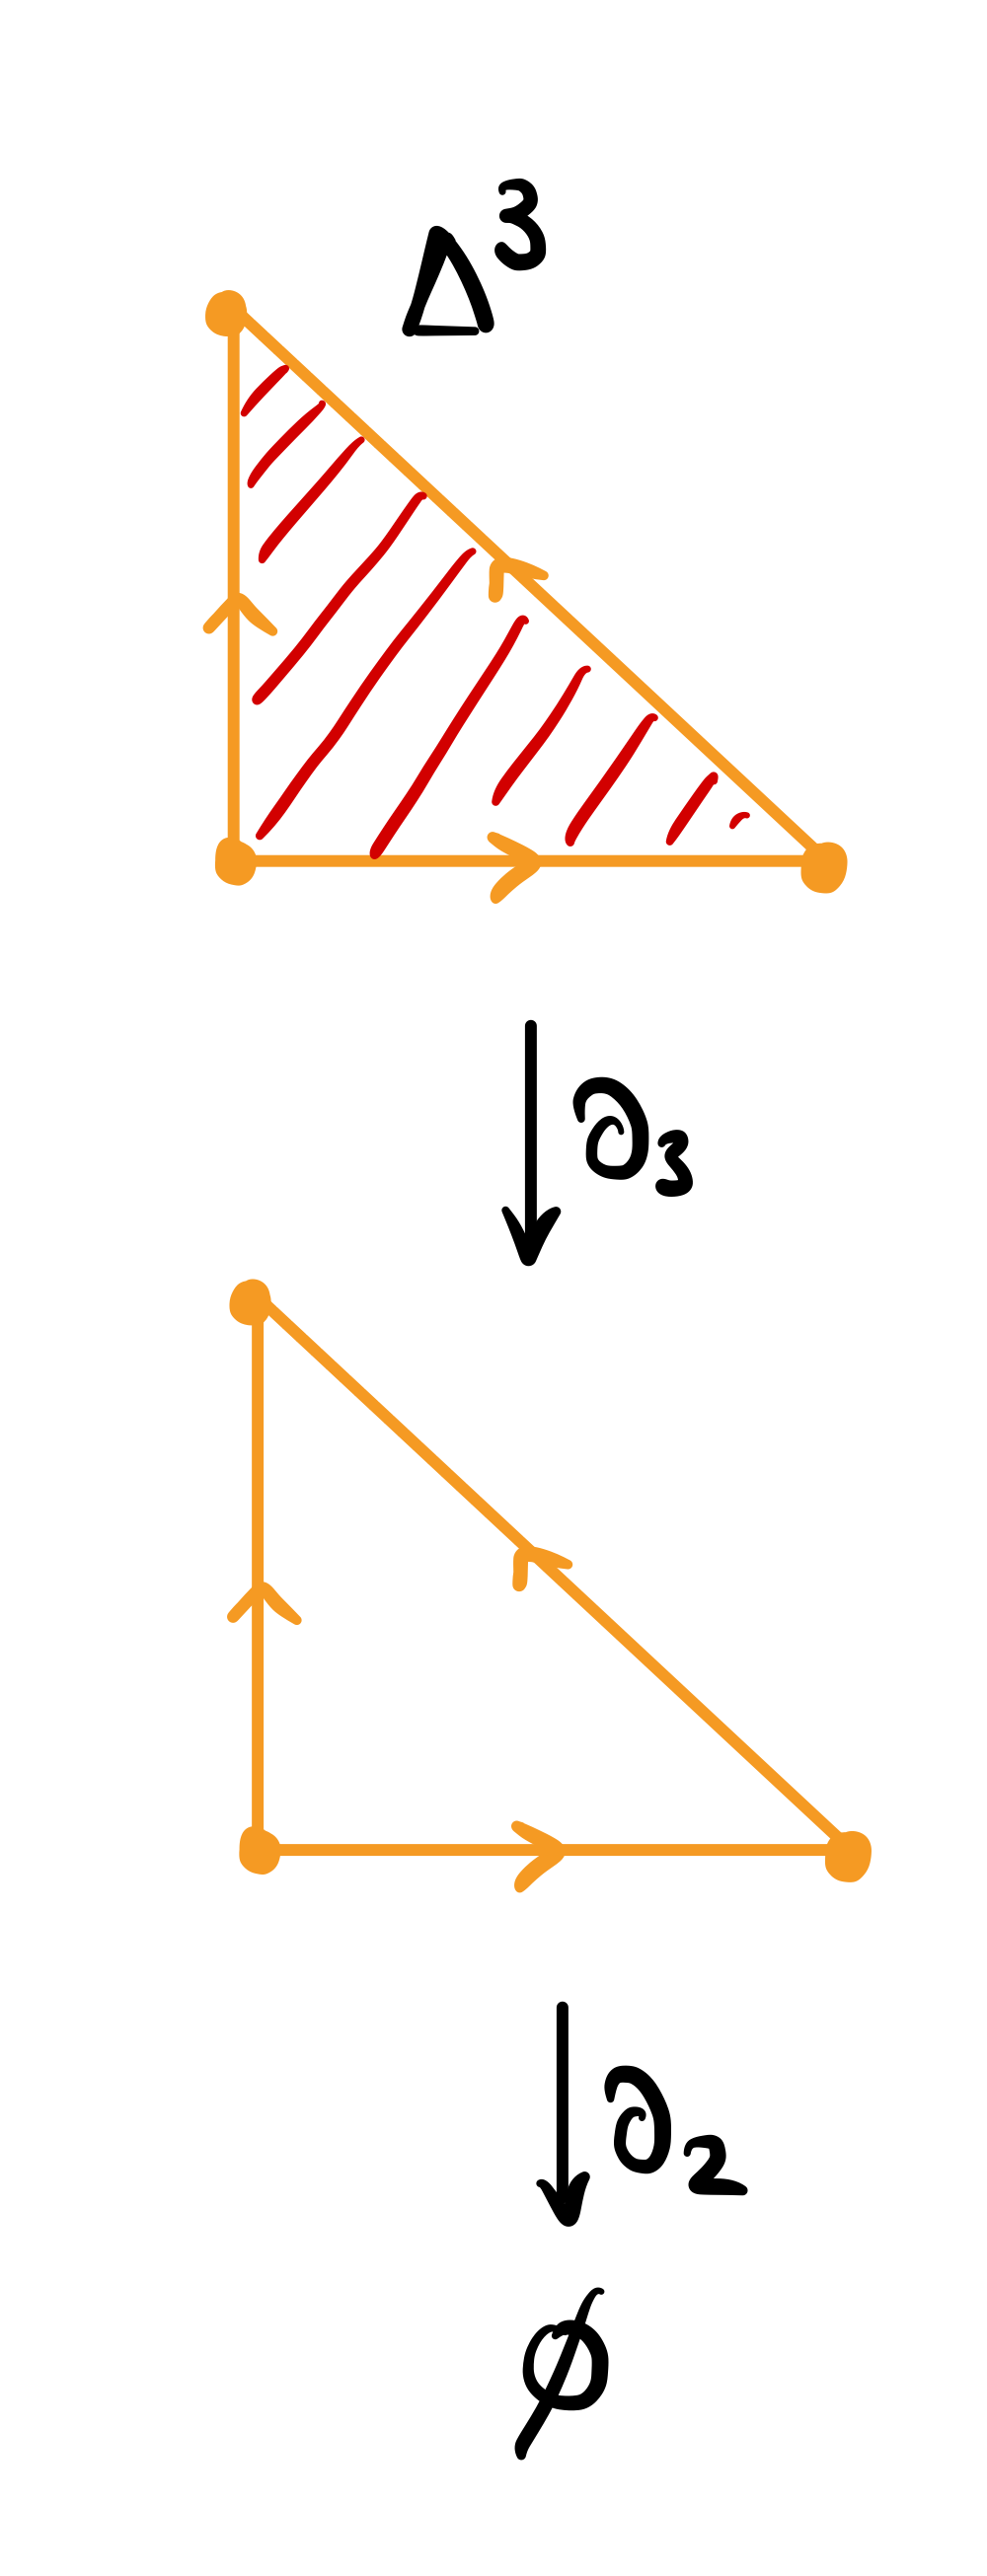
\includegraphics[scale=.08]{figures/threesimp.png}
    \caption{The face operator deletes the interior and leaves only a boundary. You can observe that a boundary has no boundary itself, so $\partial_n \circ \partial_{n-1}=0$ for all $n$.}
\end{figure}
Now we want to be able to consider many $n$-simplices at once, and we also want that two simplices which differ only in orientation cancel each other out, just like $-1+1=0$. Thus, we just allow formal sums of singular simplices with coefficients in $\mathbb{Z}$. This yields a space which we call the $n$-th chain $C_n$. The map $\partial_n$ acts linearly on each chain, yielding a so-called boundary operator $d_n: C_n \to C_{n-1}$ for each $n$.
\begin{definition}[Homology]
    \marginnote{A little reminder from MfP2: The kernel of a map consists of everything the map sends to $0$. Take for example the projection $p: \mathbb{R}^2 \to \mathbb{R}^1$ by collapsing the $y$-axis. The kernel of that map is the whole $y$-axis, so $\ker(p)=\mathbb{R}$. Also another reminder: Taking the quotient $A / B$ of a group $A$ by a subgroup $B$ (read $A$ mod $B$) means to form a new group with elements from $A$, but where all elements of $B$ are set to $0$. An example would be $\mathbb{R} / \mathbb{Z} \cong \mathbb{S}^1$. Think of gluing the real line together at all integers, so one gets infinitely many copies of $\mathbb{S}^1$, which is, of course, homeomorphic to $\mathbb{S}^1$.}
   The $n$-th homology group is given by 
   $$
   H_n(X):=\ker(\partial_n) / \text{im}(\partial_{n+1}).
   $$
\end{definition}
What does this mean? We take the kernel of the $n$-th boundary map, so everything that gets mapped to zero by $\partial_n$. Thinking in $n=2$, so paths, this means that paths without any boundary are in the kernel. This are precisely the closed paths, since an open path has its two endpoints as boundary. What is the image of $\partial_{n+1}$? This consists of paths which are boundaries of "deformed" triangles in $X$. Take for example the torus: The path wrapping around the meridian cannot be a boundary since there is no room in between the hole to have a $3$-simplex with the path as boundary. So this element is in $H_2(T)$. Same goes for the longitudinal path. The image consists of paths not wrapping around one of the holes, these are considered trivial and removed from $H_2(T)$. So we have two generators in $H_2(T)$ of infinite order. This yields heuristically $$H_2(T) \cong \mathbb{Z} \times \mathbb{Z}.$$
\begin{marginfigure}
    \centering
    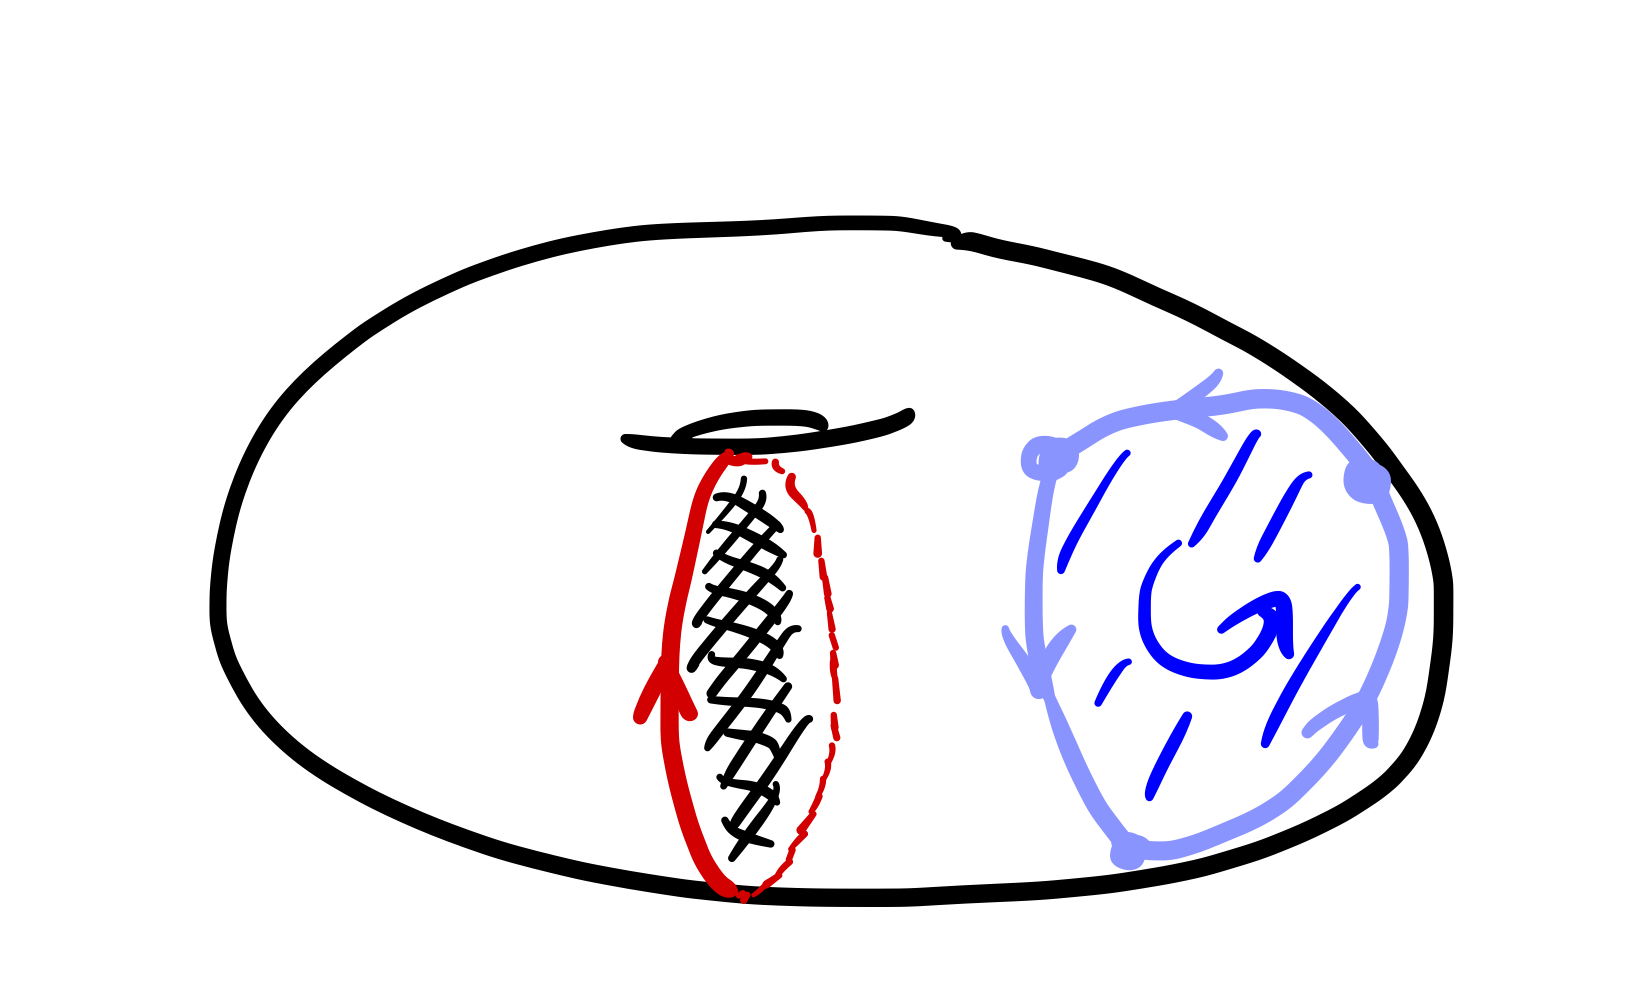
\includegraphics[scale=0.08]{figures/torus.png}
    \caption{The torus has a singular $2$-simplex visible in red which cannot possibly bound a singular $3$-simplex because of the hole. There is also another such simplex along the longitude. The blue singular $2$-simplex on the other hand is a boundary and does not contribute to homology.}
\end{marginfigure}
In higher dimensions, there is not really a nice intuition anymore. However, notice the difference to $\pi_1$: We do not demand any base point of our space. In fact, if one is concerned with counting holes of spaces, $H_n(X)$ is the way to go. Let us remark a quick sanity check for our goal:
\begin{theorem}[Hurewicz Isomorphism Theorem]
    For any top. space $X$, the map $$\pi^\text{ab}_1(X) \to H_1(X)$$ is a group isomorphism where $\pi_1^\text{ab}$ denotes the abelianzed fundamental group.
\end{theorem}
This tells us many important things:
\marginnote{There are some funny groups that vanish completely if you try to abelianize them. They are called \textbf{perfect groups}, although a lecturer of mine suggested the better fitting term Kain-ian group. One example is the alternating group $A_5$, a subgroup of the symmetric group on five letters containing only odd permutations.}
Firstly, the first homology group contains less information than the fundamental group since many things can be lost by abelianizing. This makes homology easier, but also rougher. Secondly, if we know $\pi_1$, we get many $H_1$ for free: If they are abelian, they stay just the same. Lastly, the Hurewicz map also exists for higher homotopy groups $\pi_n$, but it fails to be an isomorphism for all but $n=1$. Not everything is that nice...
